
% This LaTeX was auto-generated from MATLAB code.
% To make changes, update the MATLAB code and republish this document.

\documentclass{article}
\usepackage{graphicx}
\usepackage{color}

\sloppy
\definecolor{lightgray}{gray}{0.5}
\setlength{\parindent}{0pt}

\begin{document}

    
    
\section*{Open and plot variables from TIE-GCM netCDF files}

\begin{par}
struct m0: output from a baseline simulation w/ low F10.7 and Kp
\end{par} \vspace{1em}
\begin{par}
struct m1: output with a step-increase to Kp at t=0
\end{par} \vspace{1em}

\subsection*{Contents}

\begin{itemize}
\setlength{\itemsep}{-1ex}
   \item Load TIE-GCM output netCDF files
   \item Plot the Temperature difference (m1-m0) on a pressure level
   \item Plot the Density ratio (m1/m0) on a pressure level
   \item Plot the Density ratio (m1/m0) at a fixed altitude
   \item Plot vertical profiles of number density after 20 minutes of simulation at the location of maximum $\rho_1/\rho_0$ (from Figure 3)
   \item Plot vertical profiles of number density after 1 day of simulation at the location of maximum $\rho_1/\rho_0$ (from Figure 3)
\end{itemize}


\subsection*{Load TIE-GCM output netCDF files}

\begin{par}
m0 is the baseline simulation (low F10.7 and Kp)
\end{par} \vspace{1em}
\begin{verbatim}
m0 = get_netcdf_variables('lowF107.lowKp/s080.nc');
\end{verbatim}
\begin{par}
m1 is the "disturbed" case, in which a step function in Kp is applied at t=0
\end{par} \vspace{1em}
\begin{verbatim}
m1 = get_netcdf_variables('lowF107.lowtohighKp/s080.nc');
\end{verbatim}
\begin{par}
increase figure font size
\end{par} \vspace{1em}
\begin{verbatim}
set(0,'defaultaxesfontsize',16);
\end{verbatim}
\begin{par}
constants
\end{par} \vspace{1em}
\begin{verbatim}
boltz = 1.38e-16; % Boltzmann constant as TIE-GCM uses
m_O2=32;m_O1=16;m_N2=28;m_HE=4; % Molecular masses (AMU)
\end{verbatim}


\subsection*{Plot the Temperature difference (m1-m0) on a pressure level}

\begin{par}
Desired pressure level
\end{par} \vspace{1em}
\begin{verbatim}
nlev = 25;
\end{verbatim}
\begin{par}
loop through model output times
\end{par} \vspace{1em}
\begin{verbatim}
for it = 1:size(m0.mtime,2),
    % calculate loca time from longitude and UT time
    slt = mod([1,1/60]*double(m0.mtime(2:3,it))+m0.lon/15,24);
    % sort the data by local time
    [slt,islt] = sort(slt);
    % plot the ratio
    contourf(slt,m0.lat,(m1.TN(islt,:,nlev,it)-m0.TN(islt,:,nlev,it))',25,...
        'edgecolor','none');
    set(gca,'clim',[0,200],'xlim',[0,23.6667],'xtick',0:4:24);
    colorbar;
    % annotate plot
    xlabel('Local Time (hours)');ylabel('Latitude (deg)');
    title({'Temperature Difference (K), m1-m0',...
        sprintf('Zp=%.2f, %02d:%02d UT, Day %d',...
        m0.lev(nlev),m0.mtime([2:3,1],it))});
    % save plot
    %print(gcf,'-depsc2',sprintf('html/TNdiff_%02d',it));
end
\end{verbatim}

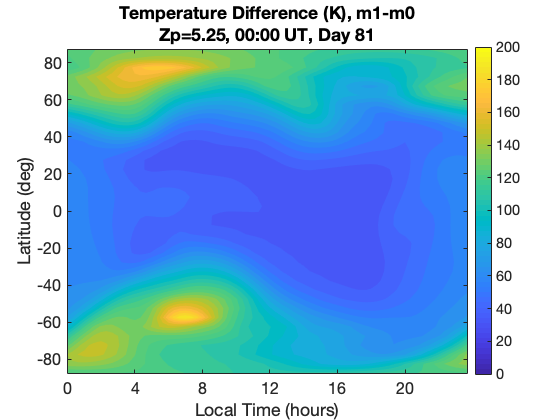
\includegraphics [width=4in]{tutorial_01.eps}
\begin{par}
Figure 1. Temperature difference $(T_1 - T_0)$ at a fixed pressure level $z_p = 5.25$.
\end{par} \vspace{1em}


\subsection*{Plot the Density ratio (m1/m0) on a pressure level}

\begin{par}
Desired pressure level
\end{par} \vspace{1em}
\begin{verbatim}
nlev = 25;
\end{verbatim}
\begin{par}
loop through model output times
\end{par} \vspace{1em}
\begin{verbatim}
for it = 1:size(m0.mtime,2),
    % calculate loca time from longitude and UT time
    slt = mod([1,1/60]*double(m0.mtime(2:3,it))+m0.lon/15,24);
    % sort the data by local time
    [slt,islt] = sort(slt);
    % plot the ratio
    contourf(slt,m0.lat,(m1.DEN(islt,:,nlev,it)./m0.DEN(islt,:,nlev,it))',25,...
        'edgecolor','none');
    set(gca,'clim',[0.9,1],'xlim',[0,23.6667],'xtick',0:4:24);
    colorbar
    % annotate plot
    xlabel('Local Time (hours)');ylabel('Latitude (deg)');
    title({'Density Ratio, m1/m0',...
        sprintf('Zp=%.2f, %02d:%02d UT, Day %d',...
        m0.ilev(nlev),m0.mtime([2:3,1],it))});
    % save plot
    %print(gcf,'-depsc2',sprintf('html/DENratio_%02d',it));
end
\end{verbatim}

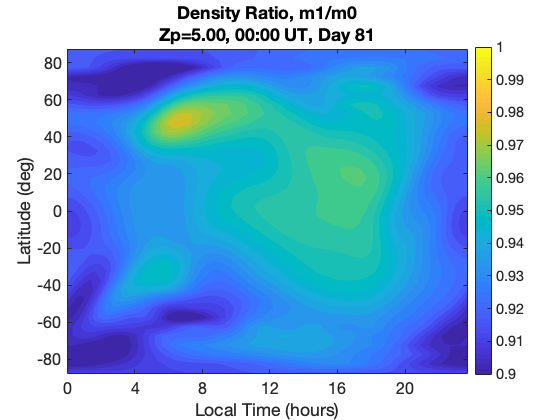
\includegraphics [width=4in]{tutorial_02.eps}
\begin{par}
Figure 2. Density ratio $(\rho_1/\rho_0)$ at a fixed pressure level $z_p = 5.0$.
\end{par} \vspace{1em}


\subsection*{Plot the Density ratio (m1/m0) at a fixed altitude}

\begin{par}
Desired height
\end{par} \vspace{1em}
\begin{verbatim}
height = 400e5; % (cm)
\end{verbatim}
\begin{par}
loop through model output times
\end{par} \vspace{1em}
\begin{verbatim}
for it = 1:size(m0.mtime,2),
    % calculate loca time from longitude and UT time
    slt = mod([1,1/60]*double(m0.mtime(2:3,it))+m0.lon/15,24);
    % sort the data by local time
    [slt,islt] = sort(slt);
    % interpolate to fixed altitude in log-space
    [m0.den_alt,m1.den_alt] = deal(zeros(length(m0.lon),length(m0.lat))); % preallocate to avoid variables growing in for-loop
    for ilon = 1:length(m0.lon),
        for ilat = 1:length(m0.lat),
            m0.den_alt(ilon,ilat) = interp1q(squeeze(m0.ZG(ilon,ilat,1:end-1,it)),log(squeeze(m0.DEN(ilon,ilat,1:end-1,it))),height);
            m1.den_alt(ilon,ilat) = interp1q(squeeze(m1.ZG(ilon,ilat,1:end-1,it)),log(squeeze(m1.DEN(ilon,ilat,1:end-1,it))),height);
        end
    end
    % convert log-densities back to densities
    [m0.den_alt,m1.den_alt] = deal(exp(m0.den_alt),exp(m1.den_alt));
    % plot the ratio
    contourf(slt,m0.lat,(m1.den_alt(islt,:)./m0.den_alt(islt,:))',25,...
        'edgecolor','none');
    set(gca,'clim',[1,1.65],'xlim',[0,23.6667],'xtick',0:4:24);
    colorbar
    % annotate plot
    xlabel('Local Time (hours)');ylabel('Latitude (deg)');
    title({'Density Ratio, m1/m0',...
        sprintf('Height = %d km, %02d:%02d UT, Day %d',...
        round(1e-5*height),m0.mtime([2:3,1],it))});
    % save plot
    %print(gcf,'-depsc2',sprintf('html/DENratio_alt_%02d',it));
end
\end{verbatim}

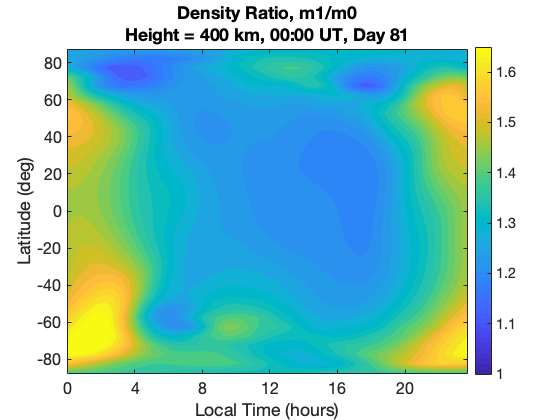
\includegraphics [width=4in]{tutorial_03.eps}
\begin{par}
Figure 3. Density ratio $(\rho_1/\rho_0)$ at a fixed altitude of 400 km.
\end{par} \vspace{1em}


\subsection*{Plot vertical profiles of number density after 20 minutes of simulation at the location of maximum $\rho_1/\rho_0$ (from Figure 3)}

\begin{par}
Starting with the ideal gas law, we want to calculate number density for species $i$:
\end{par} \vspace{1em}
\begin{par}
$$ P = n k_B T $$
\end{par} \vspace{1em}
\begin{par}
Substitute $\rho = n \bar{m}$
\end{par} \vspace{1em}
\begin{par}
$$ P = \frac{\rho}{\bar{m}} k_B T $$
\end{par} \vspace{1em}
\begin{par}
Multiply both sides by the mass mixing ratio of species $i$:
\end{par} \vspace{1em}
\begin{par}
$$ \psi_i P = \frac{\psi_i \rho}{\bar{m}} k_B T $$
\end{par} \vspace{1em}
\begin{par}
Substitute $\psi_i \rho = \rho_i = n_i m_i$:
\end{par} \vspace{1em}
\begin{par}
$$ \psi_i P = \frac{n_i m_i}{\bar{m}} k_B T $$
\end{par} \vspace{1em}
\begin{par}
Solve for number density $n_i$ in terms of TIE-GCM output variables:
\end{par} \vspace{1em}
\begin{par}
$$ n_i = \frac{\psi_i P \bar{m}}{m_i k_B T} $$
\end{par} \vspace{1em}
\begin{verbatim}
it = 1; % time index
\end{verbatim}
\begin{par}
calculate local time
\end{par} \vspace{1em}
\begin{verbatim}
slt = mod([1,1/60]*double(m0.mtime(2:3,it))+m0.lon/15,24);
\end{verbatim}
\begin{par}
find maximum density difference from previous plot after 1 day of simulation
\end{par} \vspace{1em}
\begin{verbatim}
[ilon,ilat] = find( max(max(m1.den_alt./m0.den_alt)) == m1.den_alt./m0.den_alt );
\end{verbatim}
\begin{par}
Calculate pressure on the midpoints (lev) as opposed to interfaces (ilev) for these variables:
\end{par} \vspace{1em}
\begin{verbatim}
P = m0.p0_model*exp(-m0.lev);
\end{verbatim}
\begin{par}
Calculate mean mass $\bar{m}$ for baseline model m0
\end{par} \vspace{1em}
\begin{verbatim}
m0.HE = 1-m0.O2-m0.O1-m0.N2; % quick fix: I forgot to output HE in these files, woops
m0.mbar = 1./(m0.O2/32+m0.O1/16+m0.N2/28+m0.HE/4);
\end{verbatim}
\begin{par}
Calculate $n_i$ for baseline model m0 (ignore the upper 4 grid points for composition)
\end{par} \vspace{1em}
\begin{verbatim}
term = (1/boltz)*P(1:end-4).*squeeze(m0.mbar(ilon,ilat,1:end-4,it)./m0.TN(ilon,ilat,1:end-4,it));
m0.n_O2 = term.*squeeze(m0.O2(ilon,ilat,1:end-4,it))/m_O2;
m0.n_O1 = term.*squeeze(m0.O1(ilon,ilat,1:end-4,it))/m_O1;
m0.n_N2 = term.*squeeze(m0.N2(ilon,ilat,1:end-4,it))/m_N2;
m0.n_HE = term.*squeeze(m0.HE(ilon,ilat,1:end-4,it))/m_HE;
\end{verbatim}
\begin{par}
Calculate mean mass $\bar{m}$ for disturbed model m1
\end{par} \vspace{1em}
\begin{verbatim}
m1.HE = 1-m1.O2-m1.O1-m1.N2; % quick fix: I forgot to output HE in these files, woops
m1.mbar = 1./(m1.O2/32+m1.O1/16+m1.N2/28+m1.HE/4);
\end{verbatim}
\begin{par}
Calculate $n_i$ for disturbed model m1 (ignore the upper 4 grid points for composition)
\end{par} \vspace{1em}
\begin{verbatim}
term = (1/boltz)*P(1:end-4).*squeeze(m1.mbar(ilon,ilat,1:end-4,it)./m1.TN(ilon,ilat,1:end-4,it));
m1.n_O2 = term.*squeeze(m1.O2(ilon,ilat,1:end-4,it))/m_O2;
m1.n_O1 = term.*squeeze(m1.O1(ilon,ilat,1:end-4,it))/m_O1;
m1.n_N2 = term.*squeeze(m1.N2(ilon,ilat,1:end-4,it))/m_N2;
m1.n_HE = term.*squeeze(m1.HE(ilon,ilat,1:end-4,it))/m_HE;
\end{verbatim}
\begin{par}
plot m0 and m1 profiles
\end{par} \vspace{1em}
\begin{verbatim}
subplot 121
semilogx([m0.n_O2,m0.n_O1,m0.n_N2,m0.n_HE],1e-5*squeeze(m0.ZGMID(ilon,ilat,1:end-4,it)),'--','linewidth',1);
hold on;
set(gca,'colororderindex',1);
semilogx([m1.n_O2,m1.n_O1,m1.n_N2,m1.n_HE],1e-5*squeeze(m1.ZGMID(ilon,ilat,1:end-4,it)),'linewidth',1);
xlabel('Number Density (1/cm^3)');
ylabel('Height (km)');
title({'20 Minutes After Onset',sprintf('Lon=%d, Lat=%.1f',m0.lon(ilon),m0.lat(ilat))});
xlim([1e6,1e10])
ylim([100,550]);
legend('O_2','O','N_2','He');
\end{verbatim}

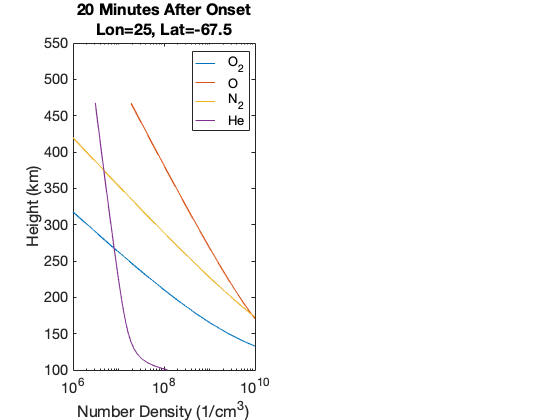
\includegraphics [width=4in]{tutorial_04.eps}


\subsection*{Plot vertical profiles of number density after 1 day of simulation at the location of maximum $\rho_1/\rho_0$ (from Figure 3)}

\begin{par}
Starting with the ideal gas law, we want to calculate number density for species $i$:
\end{par} \vspace{1em}
\begin{par}
$$ P = n k_B T $$
\end{par} \vspace{1em}
\begin{par}
Substitute $\rho = n \bar{m}$
\end{par} \vspace{1em}
\begin{par}
$$ P = \frac{\rho}{\bar{m}} k_B T $$
\end{par} \vspace{1em}
\begin{par}
Multiply both sides by the mass mixing ratio of species $i$:
\end{par} \vspace{1em}
\begin{par}
$$ \psi_i P = \frac{\psi_i \rho}{\bar{m}} k_B T $$
\end{par} \vspace{1em}
\begin{par}
Substitute $\psi_i \rho = \rho_i = n_i m_i$:
\end{par} \vspace{1em}
\begin{par}
$$ \psi_i P = \frac{n_i m_i}{\bar{m}} k_B T $$
\end{par} \vspace{1em}
\begin{par}
Solve for number density $n_i$ in terms of TIE-GCM output variables:
\end{par} \vspace{1em}
\begin{par}
$$ n_i = \frac{\psi_i P \bar{m}}{m_i k_B T} $$
\end{par} \vspace{1em}
\begin{verbatim}
it = 72; % time index
\end{verbatim}
\begin{par}
calculate local time
\end{par} \vspace{1em}
\begin{verbatim}
slt = mod([1,1/60]*double(m0.mtime(2:3,it))+m0.lon/15,24);
\end{verbatim}
\begin{par}
find maximum density difference from previous plot after 1 day of simulation
\end{par} \vspace{1em}
\begin{verbatim}
[ilon,ilat] = find( max(max(m1.den_alt./m0.den_alt)) == m1.den_alt./m0.den_alt );
\end{verbatim}
\begin{par}
Calculate pressure on the midpoints (lev) as opposed to interfaces (ilev) for these variables:
\end{par} \vspace{1em}
\begin{verbatim}
P = m0.p0_model*exp(-m0.lev);
\end{verbatim}
\begin{par}
Calculate mean mass $\bar{m}$ for baseline model m0
\end{par} \vspace{1em}
\begin{verbatim}
m0.HE = 1-m0.O2-m0.O1-m0.N2; % quick fix: I forgot to output HE in these files, woops
m0.mbar = 1./(m0.O2/32+m0.O1/16+m0.N2/28+m0.HE/4);
% Calculate $n_i$ for baseline model m0 (ignore the upper 4 grid points for composition)
term = (1/boltz)*P(1:end-4).*squeeze(m0.mbar(ilon,ilat,1:end-4,it)./m0.TN(ilon,ilat,1:end-4,it));
m0.n_O2 = term.*squeeze(m0.O2(ilon,ilat,1:end-4,it))/m_O2;
m0.n_O1 = term.*squeeze(m0.O1(ilon,ilat,1:end-4,it))/m_O1;
m0.n_N2 = term.*squeeze(m0.N2(ilon,ilat,1:end-4,it))/m_N2;
m0.n_HE = term.*squeeze(m0.HE(ilon,ilat,1:end-4,it))/m_HE;
\end{verbatim}
\begin{par}
Calculate mean mass $\bar{m}$ for disturbed model m1
\end{par} \vspace{1em}
\begin{verbatim}
m1.HE = 1-m1.O2-m1.O1-m1.N2; % quick fix: I forgot to output HE in these files, woops
m1.mbar = 1./(m1.O2/32+m1.O1/16+m1.N2/28+m1.HE/4);
\end{verbatim}
\begin{par}
Calculate $n_i$ for disturbed model m1 (ignore the upper 4 grid points for composition)
\end{par} \vspace{1em}
\begin{verbatim}
term = (1/boltz)*P(1:end-4).*squeeze(m1.mbar(ilon,ilat,1:end-4,it)./m1.TN(ilon,ilat,1:end-4,it));
m1.n_O2 = term.*squeeze(m1.O2(ilon,ilat,1:end-4,it))/m_O2;
m1.n_O1 = term.*squeeze(m1.O1(ilon,ilat,1:end-4,it))/m_O1;
m1.n_N2 = term.*squeeze(m1.N2(ilon,ilat,1:end-4,it))/m_N2;
m1.n_HE = term.*squeeze(m1.HE(ilon,ilat,1:end-4,it))/m_HE;
\end{verbatim}
\begin{par}
plot m0 and m1 profiles
\end{par} \vspace{1em}
\begin{verbatim}
subplot 122
semilogx([m0.n_O2,m0.n_O1,m0.n_N2,m0.n_HE],1e-5*squeeze(m0.ZGMID(ilon,ilat,1:end-4,it)),'--','linewidth',1);
hold on;
set(gca,'colororderindex',1);
semilogx([m1.n_O2,m1.n_O1,m1.n_N2,m1.n_HE],1e-5*squeeze(m1.ZGMID(ilon,ilat,1:end-4,it)),'linewidth',1);
xlabel('Number Density (1/cm^3)');
ylabel('Height (km)');
title({'1 Day After Onset',sprintf('Lon=%d, Lat=%.1f',m0.lon(ilon),m0.lat(ilat))});
xlim([1e6,1e10])
ylim([100,550]);
legend('O_2','O','N_2','He');
\end{verbatim}

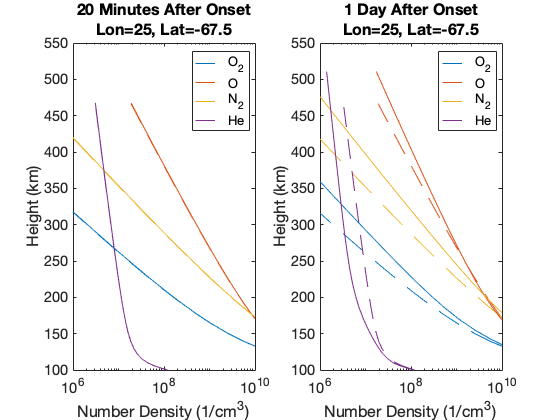
\includegraphics [width=4in]{tutorial_05.eps}



\end{document}
    
